% Versión para diapositiva (plantilla Semana ICG 2026): tamaño real 1:1, texto de 24 pt.
% Componentes de un mosaico SAR según Liu et al. (2024). Insertar en PowerPoint al 100 %.
\documentclass[border=2pt]{standalone}
\usepackage{iftex}
\ifPDFTeX
  \usepackage[utf8]{inputenc}
  \usepackage[T1]{fontenc}
  \usepackage[sfdefault]{carlito}
\else
  \usepackage{fontspec}
  \setmainfont{Carlito}[Extension=.ttf, UprightFont=*-Regular, BoldFont=*-Bold,
    ItalicFont=*-Italic, BoldItalicFont=*-BoldItalic]
\fi
\usepackage{tikz}
\usetikzlibrary{arrows.meta, positioning}

\definecolor{tinta}{HTML}{1B2A3A}
\definecolor{azul}{HTML}{1D5F83}
\definecolor{verde}{HTML}{5E8C45}
\definecolor{grisazul}{HTML}{7F9BB8}

\begin{document}
\fontsize{24}{29}\selectfont
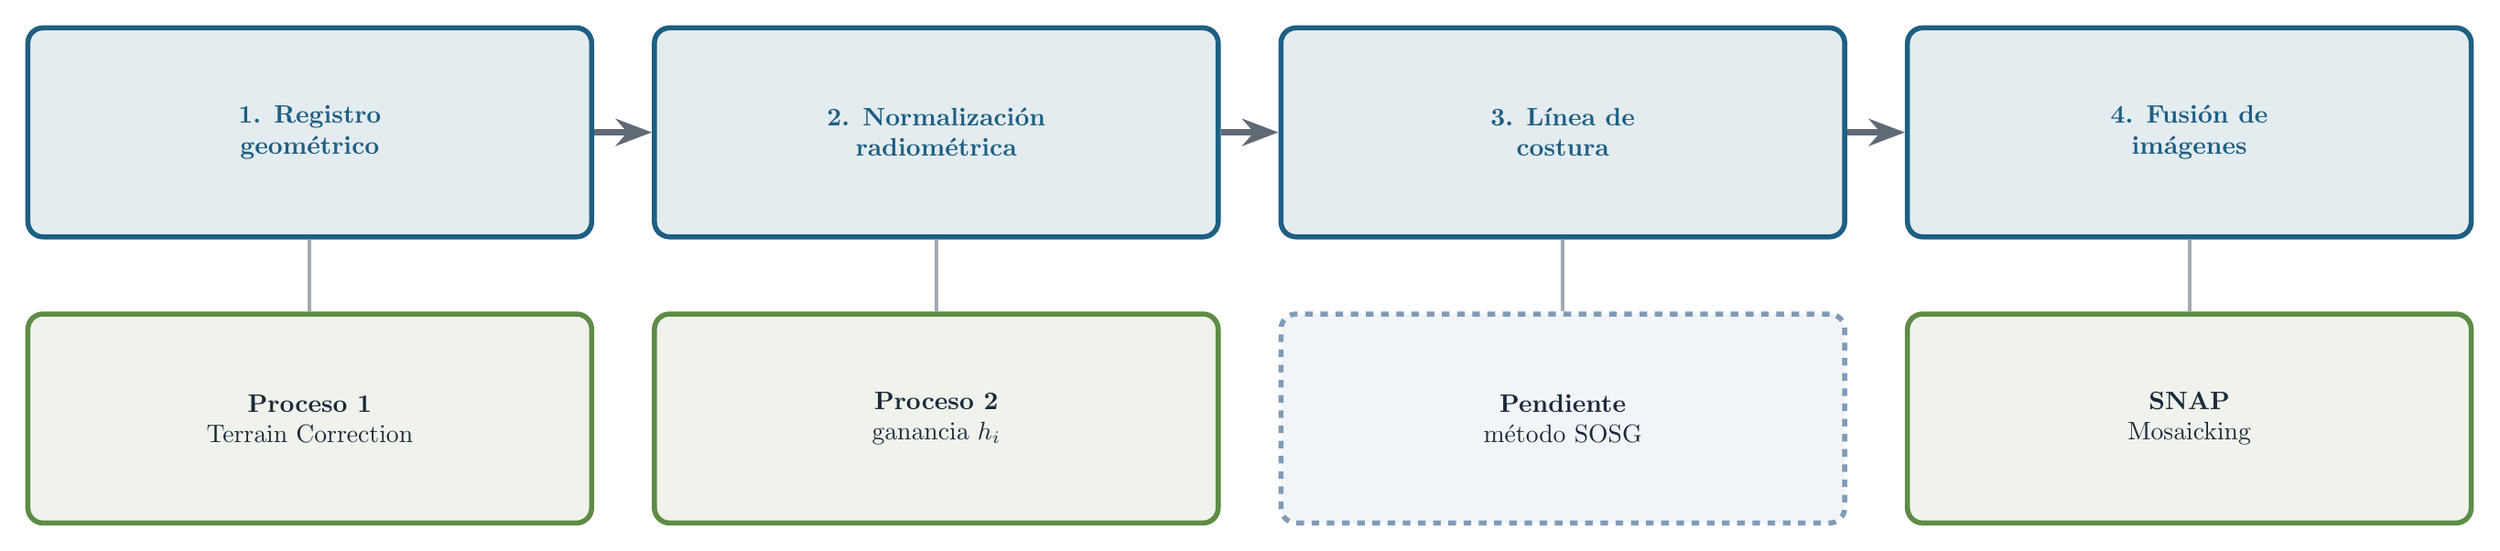
\begin{tikzpicture}[
  >=Stealth,
  comp/.style={rectangle, rounded corners=6pt, draw=azul, line width=2pt,
               fill=azul!12, text width=7.4cm, minimum height=2.9cm,
               align=flush center, text=azul, font=\bfseries, inner sep=6pt},
  si/.style={rectangle, rounded corners=6pt, draw=verde, line width=2pt,
             fill=verde!10, text width=7.4cm, minimum height=2.9cm,
             align=flush center, text=tinta, inner sep=6pt},
  no/.style={rectangle, rounded corners=6pt, draw=grisazul, dashed, line width=2pt,
             fill=grisazul!10, text width=7.4cm, minimum height=2.9cm,
             align=flush center, text=tinta, inner sep=6pt},
  flecha/.style={->, line width=2.5pt, draw=tinta!70},
  enlace/.style={line width=1.5pt, draw=tinta!40}
]
\node[comp] (c1) {1. Registro\\ geométrico};
\node[comp, right=8mm of c1] (c2) {2. Normalización\\ radiométrica};
\node[comp, right=8mm of c2] (c3) {3. Línea de\\ costura};
\node[comp, right=8mm of c3] (c4) {4. Fusión de\\ imágenes};

\foreach \a/\b in {c1/c2, c2/c3, c3/c4}
  \draw[flecha] (\a.east) -- (\b.west);

\node[si, below=10mm of c1] (e1) {\textbf{Proceso 1}\\ Terrain Correction};
\node[si, below=10mm of c2] (e2) {\textbf{Proceso 2}\\ ganancia $h_i$};
\node[no, below=10mm of c3] (e3) {\textbf{Pendiente}\\ método SOSG};
\node[si, below=10mm of c4] (e4) {\textbf{SNAP}\\ Mosaicking};

\foreach \a/\b in {c1/e1, c2/e2, c3/e3, c4/e4}
  \draw[enlace] (\a.south) -- (\b.north);
\end{tikzpicture}
\end{document}
